% !TeX root = orbits.tex
% !TeX Program=pdfLaTeX

%%%%%%%%%%%%%%%%%%%%%%%%%%%%%%%%%%%%%%%%%%%%%%%%%%%%%%%%%%%%%%%%

\pagenumbering{roman}

\thispagestyle{empty}

\begin{center}
\textbf{\LARGE The Geometry of Planetary Orbits and Ellipses}

\bigskip
\bigskip
\bigskip

\textbf{\Large Moti Ben-Ari}

\bigskip

\url{http://www.weizmann.ac.il/sci-tea/benari/}

\bigskip

Version 2.2

\bigskip

\today

\end{center}

\vspace*{8ex}

\hfill\begin{minipage}{.5\textwidth}
\small He seemed to live in some high abstract region of surds and conic sections, with little to connect him with ordinary life.
\begin{flushright}
Arthur Conan Doyle\\\textit{The Adventure of the Lion’s Mane}
\end{flushright}
\end{minipage}

\vspace*{8ex}

\hfill\begin{minipage}{.5\textwidth}
[T]his is the point at which [Feynman] finds himself unable to follow Newton's line of argument any further, and so sets out of invent one of his own \cite[p.~111]{lost}.
\end{minipage}

\vfill

\begin{center}
\copyright{} Moti Ben-Ari $2023$--$24$
\end{center}
 
\begin{small}
This work is licensed under Attribution-ShareAlike 4.0 International. To view a copy of this license, visit \url{http://creativecommons.org/licenses/by-sa/4.0/}.
\end{small}

\newpage

\tableofcontents

\newpage

\pagenumbering{arabic}

\chapter{Introduction}

Everyone ``knows'' that Kepler discovered that the orbits of the planets are ellipses and everyone ``knows'' that Newton showed that a planet in an elliptical orbit is subject to the force of gravity that is inversely proportional to the square of the distance from the Sun. Although I knew these facts, I had never seen them demonstrated until I read \textit{Calculus in Context} \cite{hahn-cic} by Alexander J. Hahn. This is a comprehensive textbook on introductory calculus that augments theory with  applications in physics and astronomy, such as the work of Kepler, Newton and Galileo, as well as applications in engineering such as building bridges and domed structures. These are not just historical anecdotes but detailed computations.

This document is a tutorial on the planetary orbits with an emphasis on proofs using Euclidean geometry. Although Newton invented the calculus and used it to study motion, from the time of the Greeks, ``proof'' meant proof by geometry. Newton's proof requires a depth of knowledge of Euclidean geometry and conic sections that is no longer studied today.

The tutorial is intended to enrich the learning of mathematics by secondary-school students and students in introductory university courses. The prerequisites are a good knowledge of Euclidean geometry along with some trigonometry, a bit calculus and Newton's laws of motions.

\section*{Overview}

Part~I of this document contains an explanation of the determination of orbits by Aristarchus, Copernicus, Kepler and Newton. The presentation is mathematical, since the historical and astronomical aspects are thoroughly described in \cite{hahn-cic}, as well as in other works. Chapter~\ref{s.aristarchus} presents the measurements of the radii of the Earth, Moon and Sun, and of the distances between them, as determined by Eratosthenes and Aristarchus. Chapter~\ref{s.copernicus} describes the construction of a model of a Sun-centered system by Nicolaus Copernicus. Chapter~\ref{s.kepler} shows how Johannes Kepler developed his three laws of planetary motion. Chapter~\ref{s.newton} presents Isaac Newton's derivation of the inverse-square law of gravitation from of Kepler's laws. One step of Newton's derivation requires a theorem whose proof is very long, so it is split off into Chapter~\ref{s.centripetal}. Even Nobel laureate Richard P. Feynman found Newton's proof daunting, so he invented his own proof which we present in Chapter~\ref{s.feynman}, along with a earlier proof by James Clerk Maxwell that uses the same technique. Chapter~\ref{s.lagrange} describes Lagrange points, points in the solar system where spacecraft can be placed so that the periods of their orbits are the same as the Earth's.

Part~II brings the definitions and theorems (and their proofs) required to understand Newton's proof. Chapter~\ref{s.definitions} contains \emph{four} definitions of ellipses and shows that the definitions are equivalent. Do not read this chapter straight through! Instead, refer to it as needed. The theorems you need to prove Newton's theorem appear in Chapter~\ref{s.ellipse}, but the proofs are in most cases modernized using analytic geometry.  Chapter~\ref{s.geometry} contains proofs of these theorems in Euclidean geometry.

Chapter~\ref{s.roulettes} is a bonus chapter on generating ellipses by roulettes and glissettes.

Theorems of Euclidean geometry that may be unfamiliar but do not concern ellipses are collected in Appendix~\ref{s.elementary}. 

\section*{Euclidean Geometry and William H. Besant}

The fundamental importance of Euclidean geometry in mathematics continued until relatively recently, as shown by this amazing quote.
\begin{quote}
In book 1, prop[osition] 10 (and notably in prop[osition] 11), Newton made use of a property of conics which he presents without proof, merely saying that the result in question comes from ``the \textit{Conics}.'' Here, as elsewhere in the \textit{Principia}, Newton assumes the reader to be familiar with the principles of conics and of Euclid. In the eighteenth and nineteenth centuries, when Newton's treatise was still being read in British universities, authors of books on ``conic sections''---for example, W. H. Besant, W. H. Drew, Isaac Milnes---supplied the proof of this theorem in order to help readers of the \textit{Principia} who might be baffled by the problem of finding a proof. They even chose letters to designate points on the diagrams so that the final result would appear in exactly the same form as in the \textit{Principia} \cite[p.~330]{newton-cohen}.
\end{quote}

William H. Besant, FRS (1828--1917) was a British mathematician who studied at Cambridge University, where he was Senior Wrangler, the student with the highest grade on the Cambridge Mathematical Tripos examination. In addition to his mathematical achievements, he was well-known as a coach for students taking the Tripos. This led to the publication of \textit{Conic Sections Treated Geometrically} in nine editions from 1869--1895.

The book has fifteen chapters, starting with a general chapter on conic sections followed by chapters on the parabola, the ellipse and the hyperbola. The chapter on ellipses has 31 propositions (theorems), 21 corollaries and 110 examples (exercises), more than you ever wanted to know about ellipses! I studied the chapter in detail and was struck by his deep knowledge of Euclidean geometry of the sort one learns in secondary school.

Project Gutenberg has published a PDF which is a transcription of the ninth edition \cite{besant}. Words like ``trigonometry,'' ``coordinate'' and ``equation'' simply do not appear.

While detailed proofs are given, Besant's style is terse, indicating that he expected his students to have an intimate familiarity with Euclidean geometry. The book has numerous diagrams (reproduced as-is in the transcription), but even the most complicated ones do not have angles and line segments labeled. This tutorial expands Besant's proofs with additional details and more elaborate diagrams.

\newpage

\section*{Newton's \textit{Principia}}

The final steps in Newton's derivation require the use of limits, which had been used already by Archimedes to compute the circumference and area of a circle by approximating the circle. Newton (along with his contemporary Gottfried Wilhelm Leibniz) developed the calculus from the concept of limits. However, the \textit{Principia} uses Euclidean geometry almost exclusively, although analytic geometry had already been developed by René Descartes and Pierre de Fermat.

The following reproduction of Newton's presentation of the infamous Book~I, Section~III, Proposition~XI, Problem~VI of the \emph{Principia} will give the reader a taste of his terse presentation. 

\smallskip
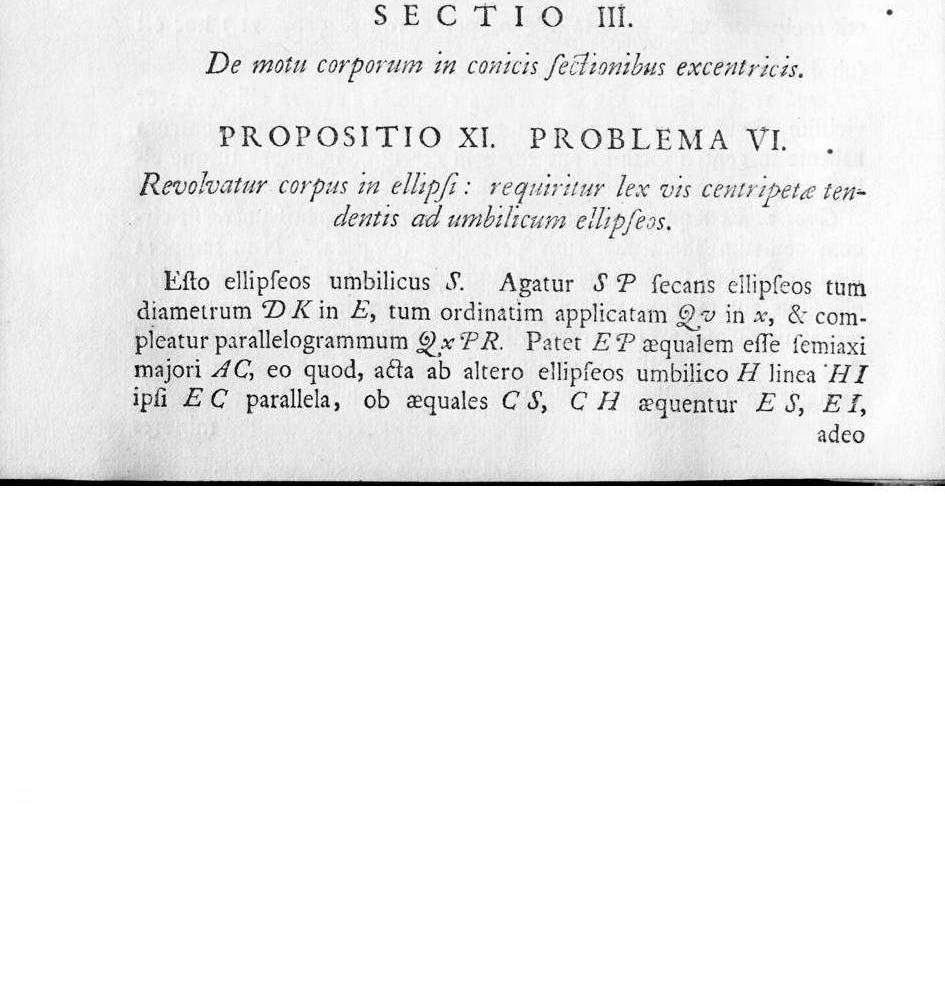
\includegraphics[width=.5\textwidth,keepaspectratio=true]{54-a.jpg}
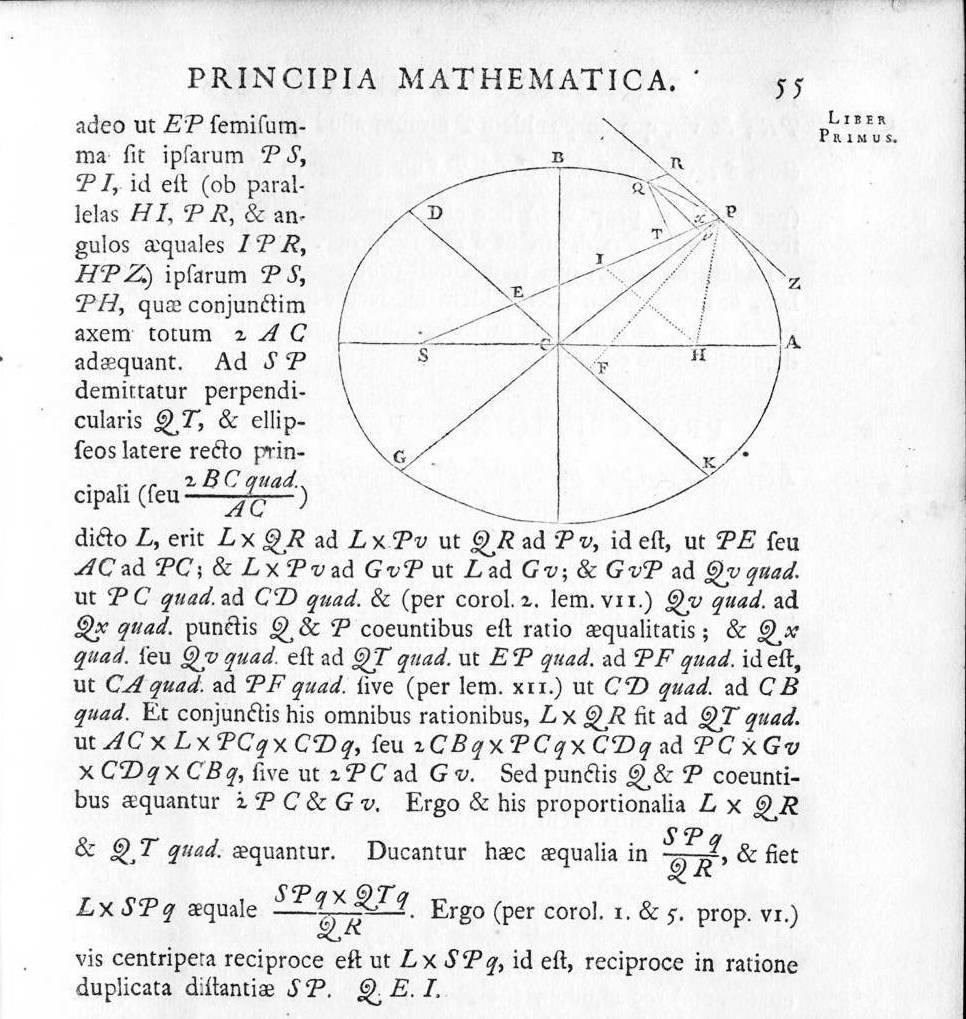
\includegraphics[width=.5\textwidth,keepaspectratio=true]{55-a.jpg}


Isaac Newton published \textit{Philosophi\ae{} Naturalis Principia Mathematica} in Latin in 1687. Subsequent editions appeared in 1723 and 1726. The third edition was translated into English as \textit{The Mathematical Principles of Natural Philosophy} by Andrew Motte in 1729. This translation has been modernized several times, but truly new translations have only appeared recently. The translation by I. Bernard Cohen is very useful because of his extensive \textit{Guide} that precedes the translation \cite{newton-cohen}.  Should you wish to attempt to understand it, a detailed explanation is given in \cite[pp.~324--329]{newton-cohen}. A comprehensive list of links to editions of the \textit{Principia} can be found in the Wikipedia entry for \textit{Philosophi\ae{} Naturalis Principia Mathematica}.

%\section{Acknowledgments}
